\begin{figure}[H]
    \centering
    \makebox[0.75\linewidth][c]{%
    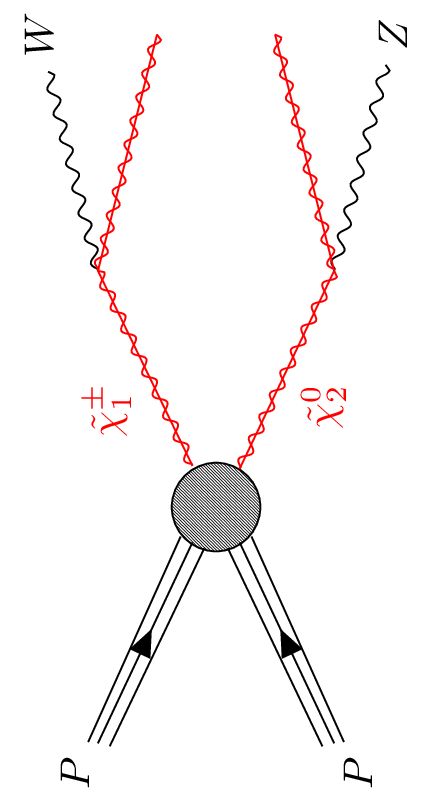
\includegraphics[width=0.225\textwidth, angle = -90]{Figures/FDiagrams/WZSignal.png}
    }
    \caption{The Feynman diagram of the signal producing a chargino-neutralino pair.}
    \label{fig:signal}
\end{figure}
\section{The Signal}\label{sec:signal}
In this thesis, I will compare \ac{ML} models in their ability to learn the patterns of the data, which will contribute  
to our ability to separate the signal from the background. Specifically for this thesis, I will be studying an expansion of the 
\ac{SM} which includes \ac{SUSY} (see section \ref{subsec:SS}). The signal I will aim to separate from the background, is one 
which produces a WZ pair, through a chargino-neutralino pair. Figure \ref{fig:signal} shows a Feynman diagram for 
such a process. The Feynman diagram shows a chargino-neutralino pair, ($\tilde{\chi}_1^\pm$ and $\tilde{\chi}_2$)
where both sparticles produce a boson (W and Z respectively) and a $\tilde{\chi}_1$, the lightest neutralino. Given that the 
neutralinos in the final state are neutral, there are three leptons and a large amount of \emph{missing transverse energy} in the final state.
In the section introducing the particle detector \ref{subsec:Detector}, I described how many of the layers rely on \ac{EM} interactions. 
Particles which only interact through the weak force are highly unlikely to interact with the detector and so in general cannot be seen. 
However, their presence can be inferred if they carry away sufficient transverse energy/momentum to measurably unbalance the event, leading to the concept of 
missing transverse energy.
